\documentclass[a4paper]{article}

%% Language and font encodings
\usepackage[english]{babel}
\usepackage[utf8x]{inputenc}
\usepackage[T1]{fontenc}

%% Sets page size and margins
\usepackage[a4paper,top=3cm,bottom=2cm,left=3cm,right=3cm,marginparwidth=1.75cm]{geometry}

%% Useful packages
\usepackage{amsmath}
\usepackage{graphicx}
\usepackage[colorinlistoftodos]{todonotes}
\usepackage[colorlinks=true, allcolors=blue]{hyperref}

\title{Introducció a la programación de lso intérpretes de comandos.}
\author{Jesús Antonio González Espinosa \\ \\ Física Computacional 1}
\date{Miércoles, 21 de Febrero del 2018}

\begin{document}
\maketitle

\section{Introducción}
Este reporte trata sobre la cuarta actividad realizada en el curso de Física Computacional 1. El objetivo de la actividad es conocer un intérprete de comandos de los sistemas operativos UNIX, en éste caso. De manera especifica, hemos hecho una primer acercamiento a las distintas formas de interactuar y hacer scripts con el Bourne Shell. Se ha trabajado con algunos comandos básicos de Bourne Shells, de los cuales se hablará durante el transcurso del reporte. 


\section{Resultados}
\subsection{Actividad}
Primero, se ha descargado un script llamado "script.sh", el cual tiene como función descargar de todos los datos de sondeos meteorológicos de un año de una estación meteorológica de la Universidad de Wyoming. Después, usamos el comando "ls -alg" para mostrar en la terminal los archivos y su tipo de permiso. Como el permiso no nos permite ejecutarlo, lo hemos cambiado con el comando "chmod". Ésta vez, al usar el comando "ls -alg", nos muestra que ya tiene permiso para ser ejecutable. 

\begin{figure}[h!]
 \centering
  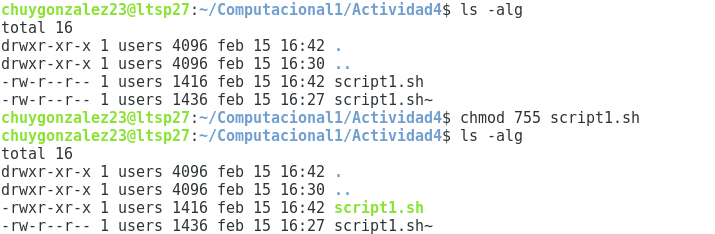
\includegraphics[width=0.6\textwidth]{PAct1.png}
\end{figure}

Ejecutamos el script, e inició una descarga de 12 archivos, uno para cada mes del año.

\begin{figure}[h!]
 \centering
  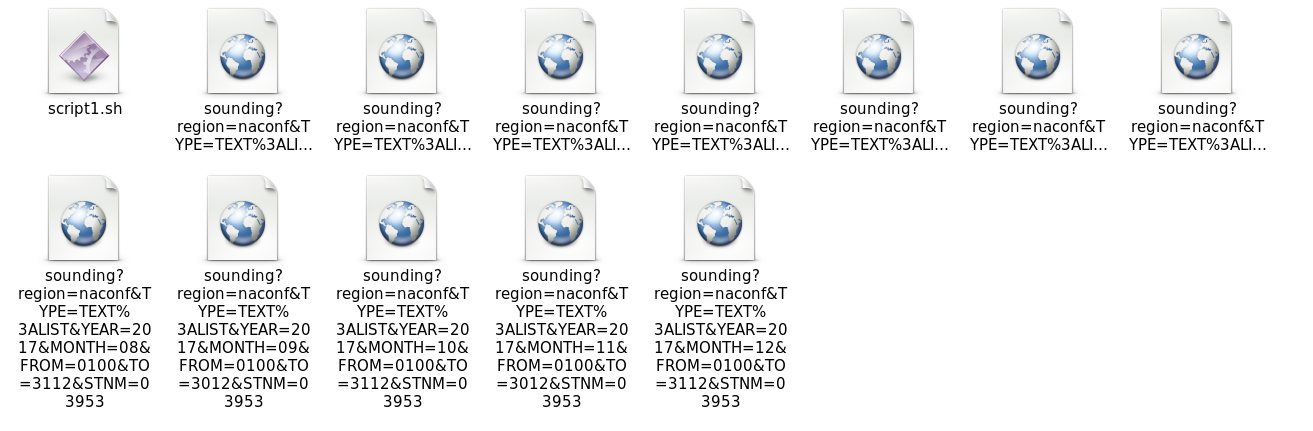
\includegraphics[width=0.6\textwidth]{PAct2.png}
\end{figure}

A continuación, se ejecutaron los comandos "less" y "cat", ambos nos permitieron observar los datos de un archivo, solo que "cat" te manda hasta el final de los datos, mientras que "less" permanecía en el inicio. Ahora la actividad introdujo el comando "grep", con el que buscamos líneas que incluyan palabras clave insertadas y muestra las muestra. Más adelante es utilizada de nuevo con otra función. Después, se analizó el tipo de archivo de los datos que se descargaron con el comando "file". Ésto mostró que todos los archivos eran de tipo texto ASCII

\begin{figure}[ht!]
 \centering
  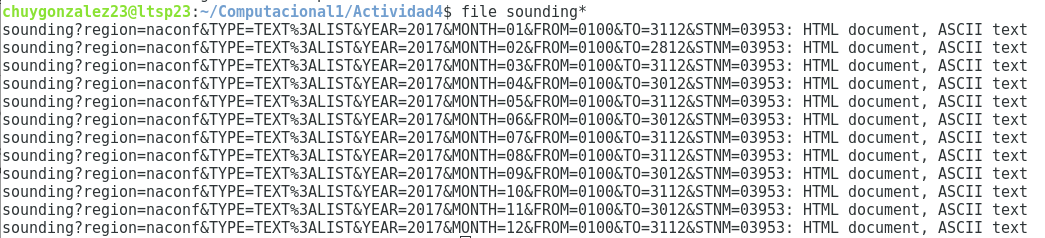
\includegraphics[width=0.8\textwidth]{PAct3.png}
\end{figure}

Ahora unimos todos los 12 archivos en uno solo, usando el comando "cat", que también permite concatenarlos en uno solo, haciendo uso de ">". Con esto, ahora tenemos el archivo "sondeos.txt", con los datos de todos los 12 meses. A continuación, hicimos uso de "grep", para filtrar los renglones de información que se quiere conservar. El comando completo fue proporcionado en la actividad. Esto crea un archivo llamado df2017.csv Después, actividad pide crear un script que haga de manera automática la concatenación de los 12 archivos y filtre los datos, cosas que hicimos a mano con los comandos. El nombre del archivo es df2017\_1.csv. 

\begin{figure}[h!]
 \centering
  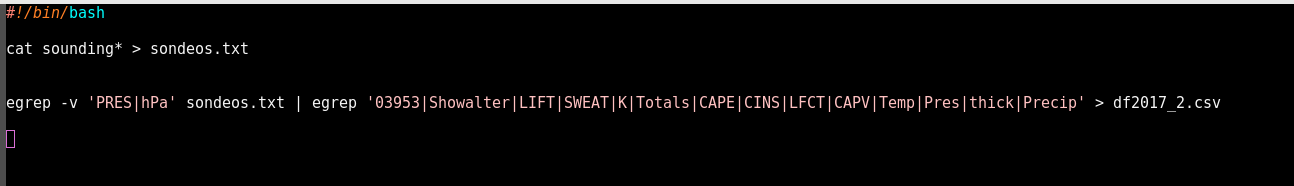
\includegraphics[width=0.8\textwidth]{PAct4.png}
\end{figure}
\begin{figure}[h!]
 \centering
  
\includegraphics[width=0.4\textwidth]{PAct5.png}
\end{figure}

Finalmente, comparamos los datos de los dos últimos archivos creados haciendo uso del comando "Diff" que nos muestra las diferencias entre ambos archivos. Como ambos tienen la misma información, ya que se hicieron con los mismos datos, el comando no muestra nada.

\begin{figure}[h!]
 \centering
  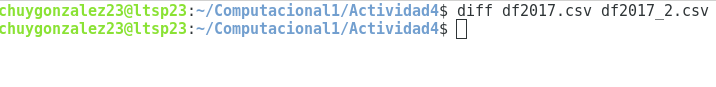
\includegraphics[width=0.8\textwidth]{PAct6.png}
\end{figure}

\subsection{Comandos}
A pesar de haber hablado un poco de los comandos en la parte anterior, aquí se explican especificamente las funciones de cada comando utilizadas en la actividad.
\begin{itemize}
\item \textbf{cat} su uso principal es para mostrar el contenido de un archivo, desde la parte final de él; esto es dentro de la terminal. Un rol secundario es para concatenar información de varios archivos en uno nuevo.
\item \textbf{chmod} sirve para cambiar los permisos de los archivos o directorios. En este se puede dar permiso a el usuario, grupo u otros, de leer, escribir o ejecutar el archivo. Utiliza la notación numérica en base 8.
\item \textbf{echo} es utilizado para la impresión de texto a en la terminal o un archivo de texto. 
\item \textbf{grep} sirve para buscar entre las líneas de un archivo, cierta palabra o caracteres claves dadas por el usuario. Otra función fue para filtrar líneas de los archivos.
\item \textbf{less} su función es parecida a "cat", ya que abre el contenido de un archivo, pero permanece hasta la parte del inicio del contenido y no te permite utilizar la terminal hasta cerrar el archivo. 
\item \textbf{ls} muestra todo el contenido del directorio. Al agregar "-alg" nos permite ver los permisos de los directorios y archivos. 
\item \textbf{wc} realiza conteos de palabras, caracteres o salto de líneas de un archivo.
\item \textbf{file} reconoce el tipo de datos que contiene un archivo. 
\item \textbf{diff} analiza dos archivos línea por línea para presentar las diferencias que hay entre ellos.
\item \textbf{Redirectores} "|" sirve para separar datos. ">" sirve para enviar información, datos o texto a un archivo.
\end{itemize}

\section{Sintesis de Shell Script Tutorial}
\subsection{Introducción}
El tutorial tiene como objetivo ayudar a la gente a comprender lo báscio de Shell Script, para introducirlos a las muchas posibilidades que ofrece el Bourne Shell. Además presenta a la audiencia a la que va dirigida el tutorial, la cual es personas con experiencia básica de programación y conocimiento en Unix/Linux Shell. 

\subsection{Filosofía}
El Shell Script tiene una mala reputación entre los sistemas Unix debido a la velocidad de interpretación en comparación a un programa en C, y la apertura a scripts de baja calidad. Es importante conocer los comandos, para poder crear y mantener un script limpio y legible. 

\subsection{Primer Script}
En esta sección se explica el inicio de un script shell. Para ejemplificarlo, se hace el clásico ejercicio de decir "Hello World". Para esto, presenta el código necesario: 
\begin{verbatim}
#!/bin/sh
# Este es un comentario!
echo Hola Mundo        # Este también es un comentario!
\end{verbatim}
La primera línea explica que el archivo va a ser ejecutado por /bin/sh. La segunda línea empieza con "\#", esto referencia una línea de comentarios; excepto en la primera línea que empieza con "\#!", que significa que lo que sigue debe ser interpretado por el Bourne Shell. La tercera línea usa el comando "echo" que nos va a imprimir en pantalla lo que sigue del comando. Por lo que al ejecutar el programa, este nos va a presentar el texto "Hola Mundo". Lo que sigue en esta sección son variaciones de éste ejemplo, como:
\begin{verbatim}
#!/bin/sh
# Este es un comentario!
echo "Hola      Mundo"       # Este también es un comentario!
\end{verbatim}
Que en este caso, imprime todo, respetando los espacios, esto se debe a las comillas, de lo cual se habla más adelante en el tutorial.

\subsection{Variables}
En esta sección se introduce a las variables. Para declarar y almacenar datos en una variable, se debe escribir y igualar al dato que se le va a depositar, ya que ve al simbolo "/=" como el comando que asigna las variables. Esto lo podemos ver en el próximo ejemplo:
\begin{verbatim}
#!/bin/sh
MY_MESSAGE="Hola mundo"
echo $MY_MESSAGE
\end{verbatim}
Lo que va a hacer es imprimir la frase "Hola mundo".

Por otra parte, al Shell no le importa el tipo de variables: enteros, reales, caracteres; mientras estás se mantengan del mismo tipo y no se intente mezclar números con letras. También se puede usar el comando "read" para leer un dato insertado de entrada y depositarlo en la variable. Al darle caracteres a una variable, es necesario ponerlo entre comillas, pero al usar el comando "read", no es necesario ya que este lo hace automáticamente. Por ejemplo:
\begin{verbatim}
#!/bin/sh
echo Cómo te llamas?
read MY_NAME
echo "Hola $MY_NAME - espero que estés bien."
\end{verbatim}
En este caso, se va a imprimir la oración, sustituyendo la variable con lo que se haya insertado en el comando "read".

Es importante recordar que las variables se reinician cada vez que ejecutamos el script. También es importante que si queremos juntar nuestra variable con otro dato, se hace entre corchetes curvos para anunciar cuando inicia y acaba la variable, para que no lo considere todo. 

\subsection{Wildcards}

En esta sección se habla de los Wildcards (comodines), que son comandos que facilitan la edición de archivos de diferentes sintaxis. 
Ejemplo:
\begin{verbatim}
#/bin/sh
cp /home/chuygonzalez23/Computacional1/Actividad4/Ayuda 
*.txt /home/chuygonzalez23/Computacional1/Actividad4
\end{verbatim}
Este ejemplo de código, lo que hace es mover un archivo desde una carpeta a otro. 
Por otra parte, el siguiente:
\begin{verbatim}
#!/bin/sh
files=`ls -1 *.txt`
for f in *.txt; do
mv "$f" "$(basename "$f" .txt).bak"
done
\end{verbatim}
Lo que hace es modificar todos los archivos con terminación .txt a .bak.

\subsection{Caracteres de Escape}

En el shell, algunos caracteres tienen un significado. En el caso de que queramos usar las comillas con el comando echo, es necesario hacer uso de la barra diagonal inversa; esto también aplica no solo para las comillas pero también para cualquier carácter especiales que shell no interpreta. Por ejemplo:
\begin{verbatim}
#!/bin/sh
echo "*"
echo "*txt"
\end{verbatim}
Aquí, va a imprimir el texto \textit{*} y \textit{*txt}
En shell, algunos caracteres tienen significados específicos, por lo que es necesario que se pongan entre comillas, para que se interpreten como texto. Por otra parte, si queremos usar las comillas como texto, es necesario usar la barra diagonal inversa; esto es necesario también con algunos caracteres como \$, \' e incluso la barra misma. Por ejemplo:
\begin{verbatim}
#!/bin/sh
echo "Esto es \" una comilla y este es \\ una barra diagonal inversa."
\end{verbatim}
\textit{Aquí lo que se va a imprimir es: Esto es " una comilla y este es \textbackslash una barra diagonal inversa.}

\subsection{Loops}
En esta sección se habla sobre los tipos de ciclos en shell. Como en cualquier otro código, los loops sirven para repetir alguna tarea varias veces. En Bourne Shell hay dos tipos,el "for" y el "while".

El primero, el "for" loop (ciclo), corre con iteraciones hasta que los valores se acaben. Por ejemplo:
\begin{verbatim}
#!/bin/sh
for i in 1 2 3 4 5
do
  echo "Ciclando ... número $i"
done
\end{verbatim}
En este ejemplo, se imprime 5 veces la oración \textit{Ciclando... número ""}, donde "" se sustituye por el número de ciclado, empezando del 1, terminando en 5.
Existen varias formas de trabajar con este tipo de ciclos, ya que los valores pueden ser palabras, archivos, letras, números, etc.

El segundo, "while" loop (ciclo), corre hasta que cumpla una condición de sálida. Por ejemplo:
\begin{verbatim}
#!/bin/sh
INPUT_STRING=hola
while [ "$INPUT_STRING" != "Adios" ]
do
  echo "Por favor escribe algo (Adios para salir)"
  read INPUT_STRING
  echo "Escribiste: $INPUT_STRING"
done
\end{verbatim}
En donde el ciclo se va a repetir, hasta que se inserte la palabra "Adios". Este tipo de ciclado puede traer más opciones.

\subsection{Test}
Los tests son para que los programas shell sean más legibles. Tiene una utilidad de comparación muy buena. 
Algunos ejemplos de los tests son:
\begin{verbatim}
#!/bin/sh
echo "Por favor adivina el número mágico: "
read X
echo $X | grep "[^0-9]" > /dev/null 2>&1
if [ "$?" -eq "0" ]; then
  # Si el grep encuentra algo diferente de 0-9
  # entonces no es un número entero.
  echo "Por favor inserta un número."
else
  # El grep encuentra solo 0-9, entonces es un entero. 
  # Podemos hacer un Test con él.
  if [ "$X" -eq "7" ]; then
    echo "Insertaste el número mágico!"
  fi
fi
\end{verbatim}
En este, pide insertar un número, si insertas el número correcto del 0 al 9, te dice que lograste encontrar el número mágico. Aquí el test revisa el número insertado.

\begin{verbatim}
#!/bin/sh
X=0
while [ -n "$X" ]
do
  echo "Ingresa algún texto (presiona Enter para salir)"
  read X
  if [ -n "$X" ]; then
    echo "Dijiste: $X"
  fi
done
\end{verbatim}
En este ejemplo, revisa que el texto insertado sea en realidad texto, si presionas enter sin escribir nada, se acaba el ciclo. 

\subsection{Case}
El comando Case ayuda para evitar muchos comandos if. Por ejemplo:
\begin{verbatim}
#!/bin/sh

echo "Por favor, habla conmigo ..."
while :
do
  read INPUT_STRING
  case $INPUT_STRING in
	hola)
		echo "Hola tú!"
		;;
	adios)
		echo "Nos vemos luego!"
		break
		;;
	*)
		echo "Lo siento, no entiendo"
		;;
  esac
done
echo 
echo "Eso es todo amigos!"
\end{verbatim}
En este caso, dependiendo de lo que insertas, el programa responde algo.

\subsection{Variables II}
Existen algunas variables que ya están puestas para el usuario y a la mayoría no se le pueden asignar valores. Estas contienen información muy útil que puede servir para que el script conozca el ambiente en el que corre. 
\begin{verbatim}
#!/bin/sh
old_IFS="$IFS"
IFS=:
echo "Por favor, una serie de tres datos separados por dos puntos ..."
read x y z
IFS=$old_IFS
echo "x es $x y es $y z es $z"
\end{verbatim}
En este ejemplo, la variable IFS, hace que las variables puedan depositar varios datos, separados por dos puntos. 

\begin{verbatim}
#!/bin/sh
/usr/local/bin/my-command
if [ "$?" -ne "0" ]; then
  echo "Perdón, hubo un problema!"
fi
\end{verbatim}
En este ejemplo, va a intentar correr un archivo, si esto se logra, va a arrojar un valor de 0, si no, va a decir que no se logró abrir el archivo.La variable \$? contiene el valor de salida del ulitmo comando que corrió.

\subsection{Variables III}
Esta sección explica como lidiar con las variables indefinidas y nulas, a partir de uso de cosas como las llaves.

\begin{verbatim}
#!/bin/sh
echo "Cuál es tu nombre? [ `whoami` ] "
read myname
if [ -z "$myname" ]; then
  myname=`whoami`
fi
echo "Tu nombre es : $myname"
\end{verbatim}
En este ejemplo, podemos ver que la línea con el comando echo, va a sustituir el 'whoami' con el nombre del usuario de la computadora; también va a imprimir lo que hay en el segundo comando echo sustiyuendo la variable con el nombre insertado. 
\subsection{Programas externos}
Los programas externos son usados regularmente con shell scripts; hay algunos comandos que vienen dentro, pero hay otros muy importantes que vienen de las utilidades de Unix.
\begin{verbatim}
#!/bin/sh
find / -name "*.html" -print | grep "/index.html$"
find / -name "*.html" -print | grep "/contents.html$"
\end{verbatim}
En este ejemplo, imprime en pantalla la información y archivos con terminación .html.

\begin{verbatim}
#!/bin/sh
HTML_FILES=`find / -name "*.html" -print`
echo "$HTML_FILES" | grep "/index.html$"
echo "$HTML_FILES" | grep "/contents.html$"
\end{verbatim}
Este ejemplo busca lo mismo, pero de manera más optimizada. 

\subsection{Funciones}
Las funciones son fáciles de usar dentro del script del Bourne Shell. La manera más sencilla de hacerlo es poniendo la función dentroo del script. Otro método es llamando una liberia al inicio del script, que contiene varias funciones muy útiles.
Una función puede devolver datos de cuatro diferentes maneras:
\begin{enumerate}
\item cambiando el estado de las variables.
\item usando el comando exit, al final para acabar todo el script.
\item usando el comando return para acabar la función y volver al script.
\item con una salida echo a una entrada estándar.
\end{enumerate}

\begin{verbatim}
#!/bin/sh

myfunc()
{
  echo "Fui llamado como : $@"
  x=2
}

### Script principal inicia aqui 

echo "Script fue llamado con $@"
x=1
echo "x es $x"
myfunc 1 2 3
echo "x es $x"
\end{verbatim}
En este ejemplo, cambia los valores de las variables.

\begin{verbatim}
#!/bin/sh

myfunc()
{
  echo "\$1 es $1"
  echo "\$2 es $2"
  # no se puede cambiar $1 - tenemos que decir:
  # 1="Adios Cruel"
  # el cual no es un syntax válido. En cambio, podemos
  # cambiar $a:
  a="Adios Cruel"
}

### Script principal inicia aquí 

a=Hola
b=Mundo
myfunc $a $b
echo "a es $a"
echo "b es $b"
\end{verbatim}
En este ejemplo también se cambia el valor de las variables.

\subsection{Pistas y Consejos}
El autor anuncia que el contenido está desactualizado; pero esta sección trata de  utilidades de manipulación de texto. Presenta varias herramientas y comandos para facilitar y optimizar la forma de trabajar con los scripts.
Ejemplo:
\begin{verbatim}
#!/bin/sh
steves=`grep -i steve /etc/passwd | cut -d: -f1`
echo "Todos los usuarios con la palabra \"steve\" en su passwd"
echo "Las entradas son: $steves"
\end{verbatim}
En este ejemplo de código, hace uso del comando grep para imprimir las entradas. El problema es que al ser varias entradas, éstas vienen en la misma línea. Un arreglo a esto es:
\begin{verbatim}
#!/bin/sh
steves=`grep -i steve /etc/passwd | cut -d: -f1`
echo "Todos los usuario con la palabra "steve" en su passwd"
echo "Las entradas son: "
echo "$steves" | tr ' ' '\012' | tr '[a-z]' '[A-Z]'
\end{verbatim}
En este código, cada entrada vienen separadas por línea; siendo una mejora al código anterior.

\pagebreak

\subsection{Quick Reference}
Esta sección incluye una guía para referencias rápidas para algunos comandos y códigos de los shell scripts. 
\begin{figure}[h!]
 \centering
  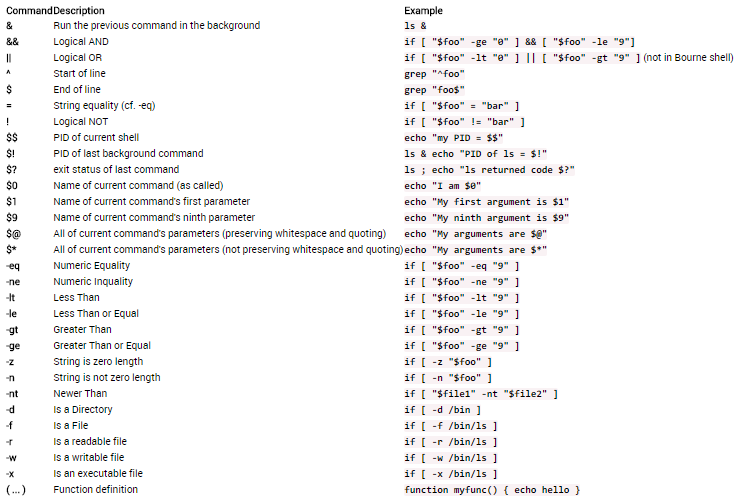
\includegraphics[width=0.8\textwidth]{SintesisQR.PNG}
\end{figure}

\subsection{Interactive Shell}
Esta sección, el autor habla de como recomienda usar el bash shell para un uso más interactivo del Unix/Linux shell. Mencionando el bash y el ksh.
El bash tiene unas herramientas de búsqueda muy útiles, facilitando el desplazamiento entre el historial de comandos previos. Por otra parte, el ksh se le pueden agregar comandos de historial. Puedes abrir una nueva sesión ksh desde otro shell interactivo, y luego volver al anterior. 

\section{Conclusión}
La actividad fue interesante e informativa, ya que fue el primer paso en cuanto a los interpretes de comandos, ya que es la priemra vez que se trabaja con shell script de forma consciente, ya que era desconocido que cuando se trabajaba con lenguajes interpretados, ya se estaban haciendo scripts. Los objetivos fueron alcanzados sin problema y la actividad realizada con éxito. 


\section{Bibliografía}
\begin{enumerate}
\item Chadwick, R. (s.f.) \textit{Bash Scripting Tutorial.} Recuperado el 23 de Febrero del 2018 desde https://ryanstutorials.net/bash-scripting-tutorial/

\item Parker, S. (2018) \textit{Shell Scripting Tutorial - The Shell Scripting Tutorial.} Recuperado el 24 de Febrero del 2018 desde https://www.shellscript.sh/index.html
\end{enumerate}

\section{Apéndice}
\begin{enumerate}
\item ¿Qué fue lo que más te llamó la atención en esta actividad?

Lo que más me llamo la atención fue conocer sobre los interpretes de comandos, el Shell Script y el Bourne Shell, 

\item ¿Qué consideras que aprendiste?

Aprendí que existe el shell scripting, ya que antes de esta actividad no sabía nada de esto. 

\item ¿Cuáles fueron las cosas que más se te dificultaron?

Nada fue muy complicado, ya había que seguir las instrucciones, pero algunos concpetos y comandos del shell script fueron difíciles de entender, pero preguntando al profesor y a los compañeros, se resolvieron tales dudas.

\item ¿Cómo se podría mejorar en esta actividad?

Tal vez con una breve explicación de los últimos incisos del resumen del tutorial de shell scripting, ya que hubo mucha dificultad para entender lo que explicaban. 


\item ¿En general, cómo te sentiste al realizar en esta actividad? 

Bien, no hubo tantas dudas, y las que hubo salieron rápido con la ayuda de internet, el resumen y/o preguntando al profesor y compañeros.

\end{enumerate}


\end{document}